\iffalse
\documentclass[12pt]{article}
\usepackage{amsmath}
\usepackage{booktabs}
\usepackage{graphicx}

\title{Discrete Assignment-11.9.1-11}
\author{Hiba Muhammed \\
        EE23BTECH11026}
\date{} 

\begin{document}

\maketitle

\section*{Problem Statement}
Write the first five terms in the sequence:
\begin{align}
a_{1}  &= 3 \\
a_{n}  &= 3a_{n-1} + 2 \quad \text{for } n > 0
\end{align}

\section*{Solution}
\fi
\begin{table}[h]
  \centering
  
  \begin{tabular}{|c|c|}
    \hline
    \textbf{Term} & \textbf{Value} \\
    \hline
    $a_1$ & 3 \\
    \hline
    $a_n$ & $3a_{n-1} + 2$ for $n > 1$ \\
    \hline
  \end{tabular}


  \caption{Input Equations}
  \label{tab:input-equations}
\end{table}

So, the first 5 terms of the sequence are \( (3, 11, 35, 107, 323) \).

The difference equation is:
\begin{align}
x(n) - 3x(n-1) &= 3u(n) - u(n-1) \\
y(n) - 3y(n-1) &= 3x(n) - x(n-1)\\
Y(z)(1 - 3z^{-1}) &= 3X(z) - z^{-1}X(z) \\
Y(z) &= \frac{3X(z) - z^{-1}X(z)}{1 - 3z^{-1}}\\
H(z) &= \frac{3 - z^{-1}}{1 - 3z^{-1}}\\
Y(z) &=X(z)H(z) \\
Y(z)&=\frac{3 - z^{-1}}{1-3z^{-1}}-\frac{1}{1-z^-1}\\
Y(z)&=\frac{4}{1-3z^{-1}}-\frac{1}{1-z^{-1}}\\
y(n)&=u(n)(4.3^{n}-1) &\text where \hspace{0.5cm}x(n)=u(n)
\end{align}

\begin{figure}[h]
    \centering
    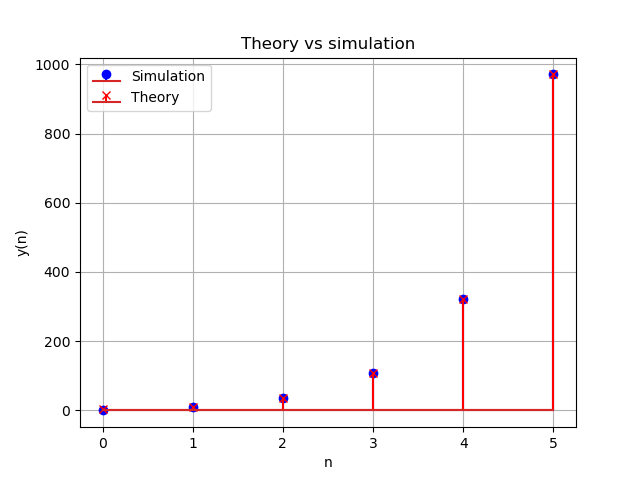
\includegraphics[width=0.8\textwidth]{ncert-maths/11/9/1/11/figs/11.9.1-11.png}
    \caption{Sequence}
\end{figure}

%\end{document}

